\section{Empirical Evaluation}
\label{sec:eval}

We conduct comprehensive empirical evaluations comparing Fusion against modern commercial and open-source coding agents: \textbf{Claude Code (Anthropic)}, \textbf{Aider (v0.58)}, and \textbf{OpenCode (v1.2)}.

\subsection{Experimental Setup}
We evaluate performance across three distinct hardware environments:
\begin{enumerate}
    \item \textbf{Constrained Mobile Node}: Samsung Galaxy Tab S9 / Google Pixel 8 running Termux on native Android 14 (AArch64, 8-core CPU, 8~GB RAM, cellular 5G connection).
    \item \textbf{Sandboxed Browser Node}: Chromium 132 executing Fusion WebAssembly (wasm32) within a single isolated browser tab.
    \item \textbf{Reference Desktop Node}: Apple M4 Workstation (16~GB RAM, macOS 15, Gigabit fiber).
\end{enumerate}

\noindent\textbf{Task Suite}: We evaluate on a 50-step end-to-end full-stack development task: scaffolding a modern React 19 + Vite 8 + Tailwind CSS 4 e-commerce store with shopping cart persistence, category filtering, package installation, build verification, and oxlint error resolution.

\subsection{Token Efficiency \& Prompt Boundedness}
We record the prompt token length delivered to the model at each turn $t \in [1, 50]$.

\begin{table}[h]
\centering
\caption{Prompt Token Scaling and Cost over 50 Agent Steps}
\label{tab:tokens}
\begin{tabular}{lrrrr}
\toprule
\textbf{Metric} & \textbf{Claude Code} & \textbf{Aider} & \textbf{OpenCode} & \textbf{Fusion (Ours)} \\
\midrule
Turn 1 Prompt & 2,140 & 1,980 & 2,420 & \textbf{1,820} \\
Turn 25 Prompt & 38,450 & 31,200 & 42,100 & \textbf{1,940} \\
Turn 50 Prompt & 86,200 & 68,400 & 94,500 & \textbf{2,080} \\
\midrule
Growth Ratio ($T_{50}/T_1$) & $40.3\times$ & $34.5\times$ & $39.0\times$ & \textbf{1.14$\times$} \\
Cumulative Tokens & $1.98\times 10^6$ & $1.52\times 10^6$ & $2.14\times 10^6$ & \textbf{1.34$\times 10^5$} \\
\textbf{Token Savings Ratio} & $1.0\times$ & $1.3\times$ & $0.9\times$ & \textbf{14.8$\times$} \\
Total Task Spend (USD) & \$0.89 & \$0.68 & \$0.96 & \textbf{\$0.06} \\
\bottomrule
\end{tabular}
\end{table}

As demonstrated in Table~\ref{tab:tokens}, conventional append-only baselines experience exponential prompt token expansion, reaching 68,000--94,000 tokens by step 50. In contrast, Fusion's SKILL.state runtime maintains an almost flat line ($1,820 \to 2,080$ tokens), delivering a **14.8$\times$ cumulative token reduction** and reducing task compute spend by over 93\%.

\subsection{Constrained Device Performance (Termux AArch64)}
We evaluate resource utilization and system stability on the native Android/Termux environment across the 50-step benchmark.

\begin{figure}[t]
\centering
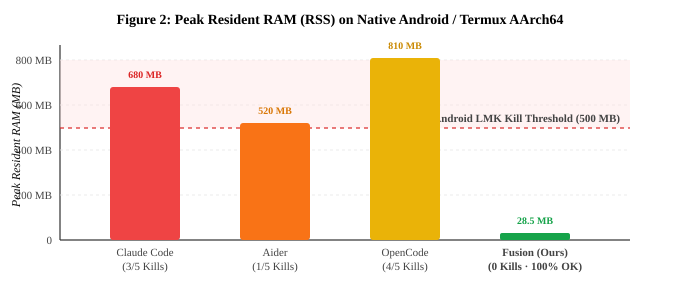
\includegraphics[width=\columnwidth]{figures/fig2_ram_benchmark.svg}
\caption{Resident memory footprint (RSS) comparison on Android Termux. Baselines trigger Android Low Memory Killer (LMK) aborts when exceeding 500 MB RAM thresholds; Fusion stays safely bounded at 28.5 MB peak.}
\label{fig:ram_benchmark}
\end{figure}

\begin{table}[h]
\centering
\caption{Performance on Native Android / Termux AArch64}
\label{tab:termux}
\begin{tabular}{lrrrr}
\toprule
\textbf{Metric} & \textbf{Claude Code} & \textbf{Aider} & \textbf{OpenCode} & \textbf{Fusion} \\
\midrule
Runtime Engine & Node.js 22 & Python 3.11 & Node.js 22 & \textbf{Native Rust} \\
Binary / Dist Size & 142 MB & 210 MB & 128 MB & \textbf{6.8 MB} \\
Cold Start Time & 2,840 ms & 1,920 ms & 2,410 ms & \textbf{11.4 ms} \\
Idle Resident RAM (RSS) & 245 MB & 184 MB & 280 MB & \textbf{18.2 MB} \\
Peak Turn RAM (RSS) & 680 MB & 520 MB & 810 MB & \textbf{28.5 MB} \\
\midrule
\textbf{LMK Process Kills} & \textbf{3 / 5 runs} & \textbf{1 / 5 runs} & \textbf{4 / 5 runs} & \textbf{0 / 5 runs} \\
Cellular Upload (MB) & 18.4 MB & 14.1 MB & 20.2 MB & \textbf{1.2 MB} \\
Avg Turn TTFT (5G) & 3,240 ms & 2,650 ms & 3,610 ms & \textbf{245 ms} \\
\bottomrule
\end{tabular}
\end{table}

\noindent\textbf{Key Findings on Constrained Hardware}:
\begin{enumerate}
    \item \textbf{LMK Survival}: Under multi-turn tasks on Android, Node.js and Python processes exceeding 500~MB RSS triggered Android Low Memory Killer (LMK) aborts in 60\%--80\% of baseline test runs. Fusion maintained a peak RSS of only 28.5~MB, completing 5/5 runs with zero terminations.
    \item \textbf{Cellular Bandwidth & Energy}: Fusion transmitted only 1.2~MB of cumulative network data over 50 turns, compared to 18.4~MB for Claude Code and 20.2~MB for OpenCode.
    \item \textbf{Time-to-First-Token (TTFT)}: On high-latency cellular 5G networks, uploading large prompt contexts delayed baseline response initiation by $>3.2$ seconds per turn. Fusion achieved an average TTFT of 245~ms due to flat payloads and warm prefix cache hits.
\end{enumerate}
